\section{Atividades}

\subsection{Atividade 1 -- Gerenciamento de Usuários e Permissões}

\paragraph{}
Inicialmente foi realizada a criação de uma nova conta local de usuário no
Windows Server 2022 utilizando as ferramentas gráficas de gerenciamento de
contas disponibilizadas pelo sistema operacional.

\paragraph{}
Durante o processo foram configurados nome de usuário, senha e permissões de
acesso necessárias para autenticação remota através do serviço de Área de
Trabalho Remota (Remote Desktop Services).

\paragraph{}
Após a criação da conta, foram realizados testes de autenticação utilizando o
novo usuário, validando seu correto funcionamento e acesso ao ambiente.

\paragraph{}
Em seguida foram realizadas alterações nas permissões da conta por meio da
adição a grupos locais do sistema, incluindo o grupo \texttt{Administrators},
permitindo compreender o impacto dos grupos de segurança na definição de
privilégios dos usuários.

\begin{figure}[H]
  \centering
  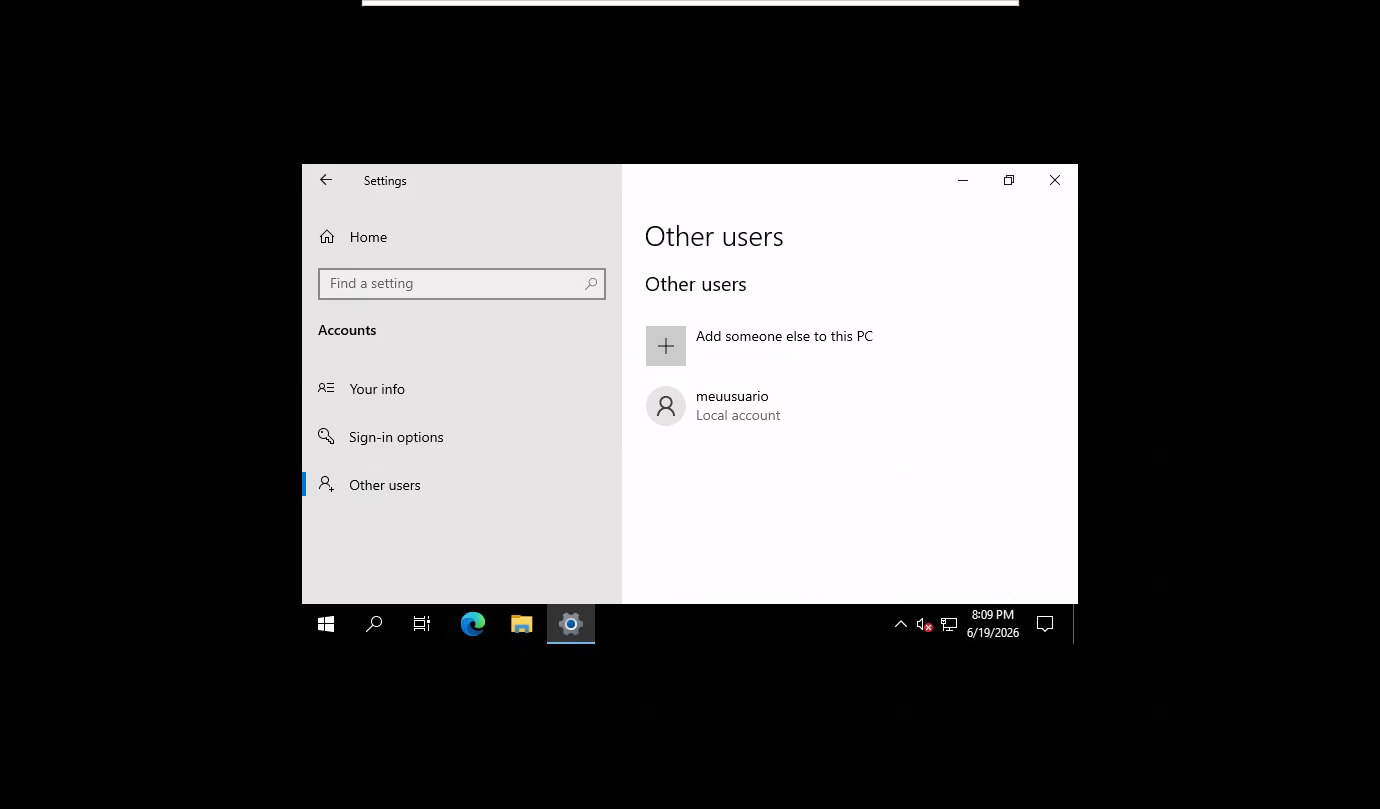
\includegraphics[width=0.95\textwidth]{./fig/usuario-criado.png}
  \caption{Conta local criada durante a atividade de gerenciamento de usuários.}
\end{figure}

\begin{figure}[H]
  \centering
  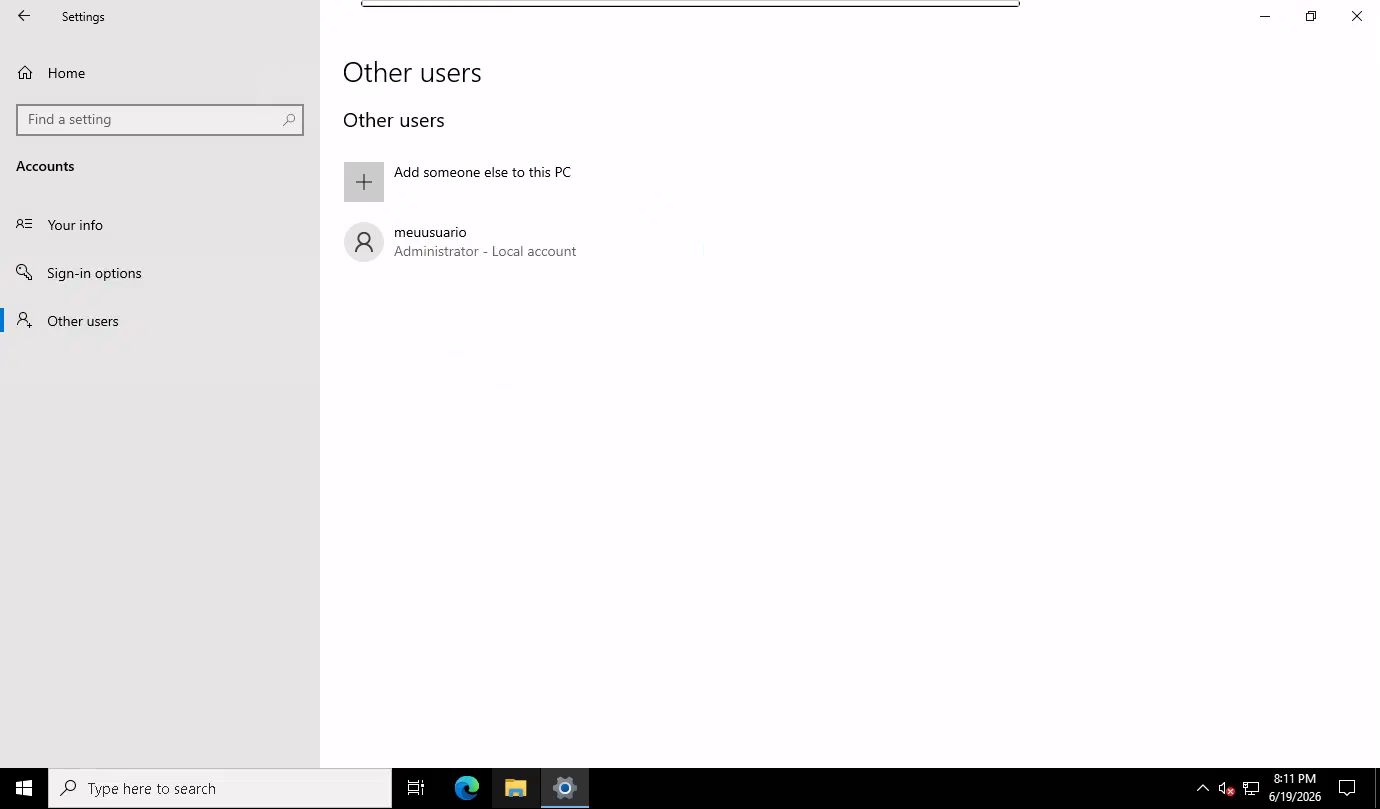
\includegraphics[width=0.95\textwidth]{./fig/usuario-administrators.png}
  \caption{Usuário adicionado ao grupo local \texttt{Administrators}.}
\end{figure}

\paragraph{}
Por fim, a conta criada foi removida do sistema, retornando o ambiente ao seu
estado original.

\subsection{Atividade 2 -- Manipulação do Registro do Windows}

\paragraph{}
Nesta atividade foi utilizada a ferramenta \texttt{Registry Editor} para
explorar a estrutura hierárquica do Registro do Windows e compreender sua
organização em chaves e valores.

\paragraph{}
Foi realizada a navegação pelas principais árvores de registro do sistema,
permitindo observar configurações relacionadas ao usuário atual e às políticas
do sistema operacional.

\paragraph{}
Durante a prática foi criada uma nova chave de configuração associada ao
\texttt{Windows Installer}, simulando a definição de uma política do sistema.

\paragraph{}
Em seguida foi criado e configurado o valor \texttt{AlwaysInstallElevated},
demonstrando como alterações no registro podem modificar o comportamento de
componentes do Windows.

\begin{figure}[H]
  \centering
  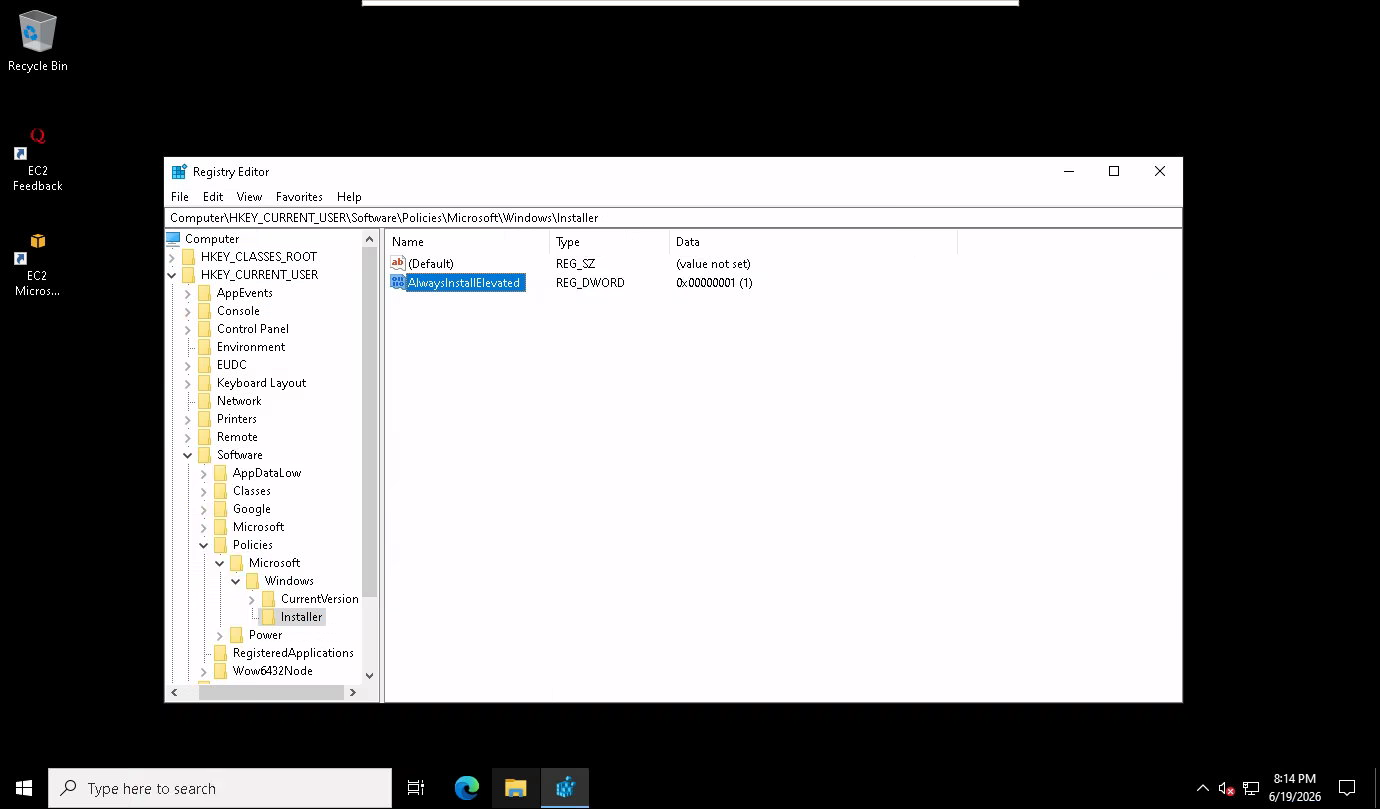
\includegraphics[width=0.95\textwidth]{./fig/always-install-elevated.png}
  \caption{Registro \texttt{AlwaysInstallElevated} configurado utilizando o
  Registry Editor.}
\end{figure}

\paragraph{}
A atividade permitiu compreender a importância do Registro como mecanismo
central de armazenamento de configurações do sistema operacional e de diversas
aplicações.

\subsection{Atividade 3 -- Gerenciamento de Serviços}

\paragraph{}
Foi realizada uma análise prática do funcionamento dos serviços do Windows
utilizando a ferramenta de linha de comando \texttt{sc.exe}.

\paragraph{}
Inicialmente foram exploradas as opções disponíveis para criação,
inicialização, consulta e remoção de serviços no sistema operacional.

\paragraph{}
Durante os testes foi criado um serviço apontando para um executável comum,
permitindo observar as restrições existentes para aplicações executadas como
serviços do Windows.

\paragraph{}
Posteriormente foi utilizada a ferramenta \texttt{msfvenom} para gerar um
executável compatível com o modelo de serviços do Windows, possibilitando a
execução de comandos administrativos durante a inicialização do serviço.

\paragraph{}
Através desse mecanismo foi realizada a criação de um usuário local e também a
adição desse usuário ao grupo \texttt{Administrators}, demonstrando como
serviços podem executar ações privilegiadas quando configurados de forma
inadequada.

\paragraph{}
Após a conclusão dos testes, os serviços e usuários criados foram removidos do
ambiente.

\subsection{Atividade 4 -- Configuração de Aplicações Startup}

\paragraph{}
Nesta etapa foi explorado o mecanismo de inicialização automática de programas
por meio da pasta \texttt{Startup} associada ao perfil do usuário.

\paragraph{}
Foi identificado o diretório responsável pelo armazenamento de atalhos de
aplicações executadas automaticamente durante o processo de login.

\paragraph{}
Em seguida foi criado um atalho para o programa \texttt{Command Prompt},
configurando sua execução automática sempre que o usuário realizasse
autenticação no sistema.

\paragraph{}
Após realizar novo login foi possível validar o funcionamento da configuração,
confirmando a execução automática da aplicação.

\paragraph{}
Por fim, o atalho foi removido da pasta \texttt{Startup}, restaurando a
configuração original do ambiente.

\subsection{Atividade 5 -- Configuração de Aplicações AutoRun}

\paragraph{}
A última atividade teve como objetivo explorar outro mecanismo de execução
automática disponível no Windows, desta vez utilizando entradas do Registro do
Sistema.

\paragraph{}
Foi realizada a navegação até a chave
\texttt{HKEY\_LOCAL\_MACHINE\textbackslash SOFTWARE\textbackslash
Microsoft\textbackslash Windows\textbackslash CurrentVersion\textbackslash
Run}, responsável por definir aplicações executadas durante a inicialização do
sistema.

\paragraph{}
Nessa chave foi criado um novo valor contendo o caminho do executável
\texttt{cmd.exe}, configurando sua execução automática após o processo de
login.

\paragraph{}
A funcionalidade foi validada por meio da realização de novo logon no sistema,
confirmando que o programa era iniciado automaticamente conforme definido no
registro.

\paragraph{}
Após os testes, o valor criado foi removido para evitar a manutenção da
configuração de execução automática.
